\documentclass[tikz]{standalone}
\usepackage{pgfplots}
\pgfplotsset{compat=1.15}
\usepackage{mathrsfs}
\usetikzlibrary{arrows,calc}
\usepackage{tkz-euclide}

\pagestyle{empty}

\definecolor{AngleClr}{rgb}{0,0.39215686274509803,0}
\definecolor{ShapeClr}{rgb}{0.6,0.2,0}

\definecolor{SecondAngleClr}{RGB}{166, 7, 7}

\begin{document}

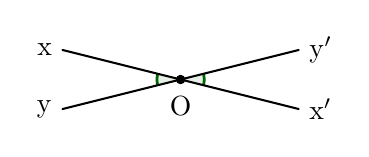
\begin{tikzpicture}[scale=.75]
\tkzSetUpLine[line width=1pt,color=black]
\tkzSetUpPoint[fill=black]

\tkzDefPoints{-2/0.5/A,2/-0.5/AA,-2/-0.5/B,2/0.5/BB}

\tkzInterLL(A,AA)(B,BB) \tkzGetPoint{O}

\tkzFillAngles[fill=AngleClr,size=.4,fill opacity=0.1](A,O,B AA,O,BB)
\tkzMarkAngles[line width=1pt,size=.4,color=AngleClr](A,O,B AA,O,BB)

\tkzDrawPoints[size=3](O)
\tkzLabelPoint[left](A){$\rm x$}
\tkzLabelPoint[right](AA){$\rm x'$}
\tkzLabelPoint[left](B){$\rm y$}
\tkzLabelPoint[right](BB){$\rm y'$}
\tkzLabelPoint[below=2.5pt](O){$\rm O$}

\tkzDrawSegments[line width=0.75pt](A,AA B,BB)

\end{tikzpicture}

\end{document}
